% !Mode:: "TeX:UTF-8"

\begin{frame}{第十讲、多元函数极限、连续与偏导数}
	\linespread{1.5}
	\begin{enumerate}
	  \item {\bf 内容与要求}{\color{blue}( \S10.1,\S10.2.1 )}
	  \begin{itemize}
	    \item 理解多元函数的概念
	    \item 掌握多元函数极限与连续的判定方法
	    \item 理解偏导数的概念及其性质
% 	    \item 熟练掌握空间平面和直线的方程
% 	    \begin{itemize}
% 	      \item 可分离变量方程
% 	      \item 齐次方程
% 	      \item 一阶线性方程
% 	    \end{itemize}
	  \vspace{1em}
	  \end{itemize}
	  \item {\bf  课后作业:}
	  \begin{itemize}
	    \item {\b 习题10.1:6,9(2,4),12(2)}
	    \item {\b 习题10.2:1(8-11),2,4,5(3,4)}
	  \end{itemize}
	\end{enumerate}
\end{frame}

\section{多元函数的概念}

\begin{frame}{什么是多元函数}
	\linespread{1.2}\pause 
	{\bf 多元}:多个变元(多个自变量)\pause 
	\begin{block}{{\bf 定义}\hfill}
		$$f:D\to\mathbb{R}\quad(D\subset\alert{\mathbb{R}^n})$$
	\end{block}\pause 
	例:
	\begin{itemize}
	  \item $z=x^2+y^2, \;((x,y)\in\mathbb{R}^2)$\pause 
	  \item $w=xyz,\;(x,y,z\geq 0)$\pause 
% 	  \item $x_n=\df{x_1x_2\ldots x_{n-1}}{x_1^2+x_2^2+\ldots+x_{n-1}^2}$
	\end{itemize}
	\begin{center}
		\ba{几何上,$n$元函数对应于$n+1$维空间中的“曲面”}
	\end{center}
\end{frame}

\begin{frame}{高维空间中的集合}
	\linespread{1.2}\pause 
	{\bb 1、邻域和去心邻域:}设$\bm{x}_0\in\mathbb{R}^n$\pause 
	$$U(\bm{x}_0,\delta)=\{\bm{x}\in\mathbb{R}^n||\bm{x}-\bm{x}_0|<\delta\}$$\pause 
	\vspace{-2em}
	$$U_0(\bm{x}_0,\delta)=U(\bm{x}_0,\delta)-\{\bm{x}_0\}$$\pause 
	{\bb 2、点$P$与点集$D$的关系}\pause 
	\begin{enumerate}
	  \item {\bf 内点:}存在邻域$U(P)\subset D$\pause 
	  \item {\bf 外点:}存在邻域$U(P)\cap D=\phi$\pause 
	  \item {\bf 边界点:}既不是内点又不是外点
	\end{enumerate}
\end{frame}

\begin{frame}
	\linespread{1.2}
	{\bb 3、点集的分类}
	\begin{enumerate}\pause 
	  \item {\bf 开集:}只有内点\pause 
	  \item {\bf 闭集:}包含所有边界点\pause 
	  \item {\bf 连通集:}集合内任意两点可以通过集合内的折线相连\pause 
	  \item {\bf 开区域:}连通的开集\pause 
	  \item {\bf 闭区域:}开区域连同其边界\pause 
	  \item {\bf 有界集:}集合可被包含于任一点的某个邻域中
	\end{enumerate}
\end{frame}

\begin{frame}
	\linespread{1.5}
	\begin{exampleblock}{{\bf 例1}\hfill}
		讨论以下集合的类型:
		\begin{enumerate}
		  \item $\{(x,y)|x^2+y^2<4\}-\{(x,y)|x^2+4(y-a)^2\leq 4\}$
		  \item $\{(x,y)|x^2+y^2<4\}-\{(x,y)||x-a|\leq 1\}$
		\end{enumerate}
	\end{exampleblock}\pause 
	\begin{exampleblock}{{\bf 例2}\hfill}
		写出下列函数的定义域:
		\begin{enumerate}
		  \item $z=\sqrt{1-x^2-y^2}$
		  \item $u=\df{1}{\sqrt{1-x^2+y^2-z^2}}$
		\end{enumerate}
	\end{exampleblock}
\end{frame}

\section{多元函数的极限与连续}

\begin{frame}{多元函数的极限}
	\linespread{1.2}\pause  
	\begin{block}{{\bf 定义10.1.3}($n$重极限)\hfill}
		{\bb $n$元函数$f(\bm{x})$在点$\bm{x}_0$处以$a$为极限:}\pause 
		
		$$\forall\e>0,\exists\delta>0,\forall \bm{x}\in U_0(\bm{x}_0,\delta),
		|f(\bm{x})-a|<\e $$\pause 
		记为
		$$\alert{\lim\limits_{\bm{x}\to\bm{x}_0}f(\bm{x})=a}$$ 
	\end{block}\pause 
	{\bf 二元函数的(二重)极限:}
	$$\alert{\lim\limits_{(x,y)\to(x_0,y_0)}f(x,y)=a}  
	\quad\mbox{或}\quad
	\alert{\lim\limits_{x\to x_0 \atop y\to y_0}f(x,y)=a}$$
\end{frame}

\begin{frame}{二重极限的几何意义}
	\linespread{1.2}\pause 
	\ba{$(x,y)$沿任意方向逼近$(x_0,y_0)$时$f(x,y)$趋于相同值}\pause 
	\begin{columns}
		\column{.5\textwidth}
		\begin{exampleblock}{{\bf 例3}\hfill}
			证明$\lim\limits_{(x,y)\to(0,0)}\df{x^2-y^2}{x^2+y^2}$不存在。\pause 
		\end{exampleblock}
		\uncover<5->{\ba{若沿不同路径所得极限不同,则二重极限不存在}}
		\column{.5\textwidth}
		\begin{center}
			\resizebox{!}{5cm}{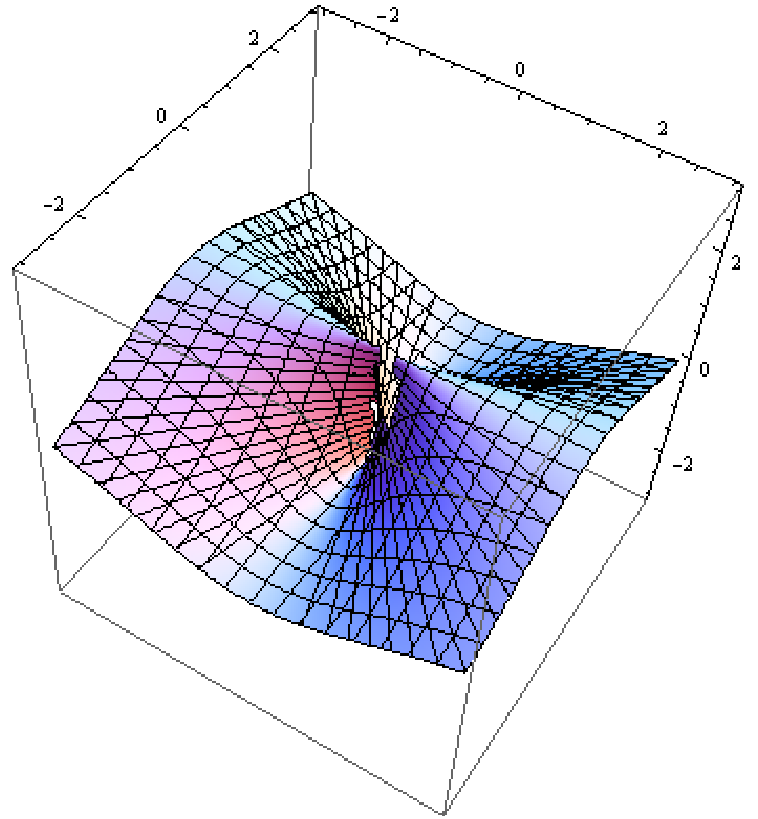
\includegraphics{./images/ch10/noLimEx.pdf}}
		\end{center}
	\end{columns}
\end{frame}

\begin{frame}
	\linespread{1.2}
	\begin{exampleblock}{{\bf 例4:}讨论以下极限\hfill}
		\begin{columns}
			\column{.5\textwidth}
				\begin{enumerate}
				  \item $\lim\limits_{(x,y)\to(0,0)}\df{x^2y}{x^2+y^2}$
% 				  \item $\lim\limits_{(x,y)\to(0,0)}\df{xy}{x^2+y^2}$
				\end{enumerate}
			\column{.5\textwidth}
				\begin{enumerate}
				  \addtocounter{enumi}{1}
				  \item $\lim\limits_{(x,y)\to(0,0)}\df{xy}{x^2+y^2}$
				\end{enumerate}
		\end{columns}
	\end{exampleblock}\pause 
	\begin{center}
		\resizebox{!}{5cm}{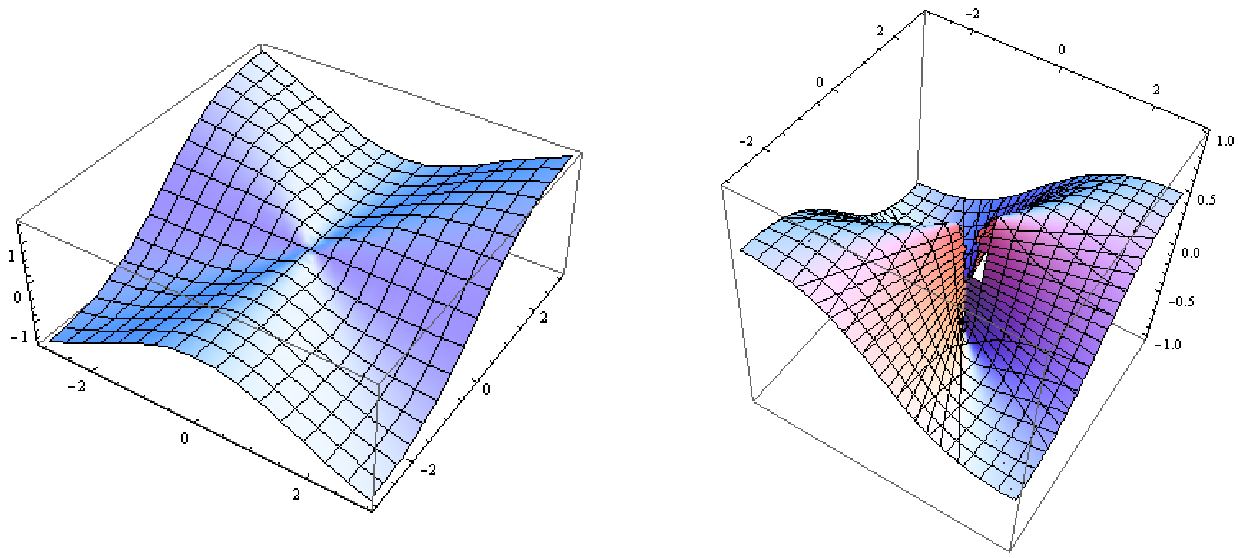
\includegraphics{./images/ch10/limEx.pdf}}
	\end{center}
\end{frame}

\begin{frame}{二重极限与累次极限}
	\linespread{1.2}\pause 
	{\bb 二重极限:}\quad $$\alert{\lim\limits_{(x,y)\to(x_0,y_0)}f(x,y)}$$
	
	\pause 
	{\bb 累次极限:}\quad $$\alert{\lim\limits_{y\to y_0}\lim\limits_{x\to
	x_0}f(x,y),\quad \lim\limits_{x\to x_0}\lim\limits_{y\to y_0}f(x,y)}$$
	\vspace{-1em}\pause 
	\begin{enumerate}
	  \item 若三者都存在,则值相等;\pause 
	  \item 二重极限存在,累次极限必存在;\pause 
	  \item 两个累次极限均存在且相等,二重极限未必存在
	\end{enumerate}
\end{frame}

\begin{frame}{多元函数的连续性}
	\linespread{1.2}\pause 
	\begin{block}{{\bf 定义10.1.4}\hfill}
		{\bb $n$元函数$f(\bm{x})$在$\bm{x}_0$处连续:}
		$$f(\bm{x}_0)=\lim\limits_{\bm{x}\to\bm{x}_0}f(\bm{x})$$
	\end{block}\pause 
	\begin{itemize}
	  \item 多元初等函数在其定义域内连续\pause 
	\end{itemize}
	\begin{exampleblock}{{\bf 例5}\hfill}
		求函数$f(x,y)=\df{\arcsin(3-x^2-y^2)}{\sqrt{x-y^2}}$连续的区域。
	\end{exampleblock}
\end{frame}

\section{偏导数}

\begin{frame}{偏导数}
	\linespread{1.2}\pause 
	\begin{block}{{\bf 定义}\hfill}
		{\bb 二元函数$z=f(x,y)$在$(x_0,y_0)$处关于$x$的偏导数:}\pause 
		\begin{eqnarray*}
			\alert{f'_x(x_0,y_0)} \pause & = &
			\left.\df{\d}{\d x}f(x,y_0)\right|_{x=x_0}\pause \\ 
			& = & \lim\limits_{x\to x_0}\df{f(x,y_0)-f(x_0,y_0)}{x-x_0}\pause \\
			& = & \alert{\left.\df{\p z}{\p x}\right|_{x=x_0,y=y_0}}
		\end{eqnarray*}
	\end{block}\pause 
	\ba{偏导数等价于将其他变量视为常数所求得的导数}
\end{frame}

\begin{frame}
	\linespread{1.2}
	$$\alert{f'_x(x_0,y_0)  =  \left.\df{\d}{\d x}f(x,y_0)\right|_{x=x_0}}$$\pause 
	\begin{exampleblock}{{\bf 例6}\hfill}
		已知$f(x,y)=x^2+2xy$,求$f'_x(-1,1)$和$f'_y(-1,1)$。
	\end{exampleblock}\pause 
	\alert{{\bf $f'_x(x_0,y_0)$的几何意义}:\pause 空间曲线
	$$\left\{\begin{array}{l}
	z=f(x,y)\\ y=y_0
	\end{array}\right.$$
	在点$(x_0,y_0,f(x_0,y_0))$处的切线关于$x$轴的斜率}
\end{frame}

\begin{frame}
	\linespread{1.2}
	\begin{exampleblock}{{\bf 例7}\hfill}
		$$f(x,y)=\left\{\begin{array}{cc}
			\df{xy}{x^2+y^2}, & (x,y)\ne (0,0)\\
			0, & else
		\end{array}\right.$$
		求$f'_x(0,0)$和$f'_y(0,0)$
	\end{exampleblock}\pause 
	\begin{itemize}
	  \item \ba{多元函数在一点偏导数存在,未必在该点连续}
	\end{itemize}
\end{frame}

\begin{frame}{偏导数的计算}
	\linespread{1.2}\pause 
	\ba{运算规则:对指定变量求导时,将其他变量视为常数}\pause 
	\begin{exampleblock}{{\bf 例8}\hfill}
		求$z=x^y$的偏导数。
	\end{exampleblock}\pause 
	\begin{exampleblock}{{\bf 例9}\hfill}
		已知$r=\sqrt{x^2+y^2+z^2}$,证明
		$$\left(\df{\p r}{\p x}\right)^2+\left(\df{\p r}{\p y}\right)^2+\left(\df{\p
		r}{\p z}\right)^2=1$$
	\end{exampleblock}
\end{frame}

\begin{frame}{高阶偏导数}
	\linespread{1.2}\pause 
	{\bb 二阶偏导数:}偏导数的偏导数\pause 
	$$\alert{f''_{xx}(x,y)=\df{\p}{\p x}\left(\df{\p z}{\p x}\right)
	=\df{\p^2 z}{\p x^2}}$$\pause 
	$$\alert{f''_{xy}(x,y)=\df{\p}{\p y}\left(\df{\p z}{\p x}\right)
	=\df{\p^2 z}{\p x\p y}}$$\pause 
	$$\alert{f''_{yy}(x,y)=\df{\p}{\p y}\left(\df{\p z}{\p y}\right)
	=\df{\p^2 z}{\p y^2}}$$\pause 
	$$\alert{f''_{yx}(x,y)=\df{\p}{\p x}\left(\df{\p z}{\p y}\right)
	=\df{\p^2 z}{\p y\p x}}$$
\end{frame}

\begin{frame}
	\linespread{1.2}
	\begin{exampleblock}{{\bf 例10}\hfill}
		验证函数$u=\sin(x-at)$满足{\bb 波动方程}
		$$\df{\p^2u}{\p t^2}=a^2\df{\p^2u}{\p x^2}$$
	\end{exampleblock}
\end{frame}

\begin{frame}{高阶偏导数的性质}
	\linespread{1.2}\pause 
	\begin{block}{{\bf 定理10.2.1}\hfill}
		若函数$z=f(x,y)$的两个混合偏导函数$f''_{xy}(x,y)$和$f''_{yx}(x,y)$
		均在$(x_0,y_0)$处连续,则
		$$f''_{xy}(x_0,y_0)=f''_{yx}(x_0,y_0)$$
	\end{block}\pause 
	\begin{itemize}
	  \item 定理结论可推广到高阶偏导数的情形\pause 
	  \item \alert{求初等函数的高阶偏导数可任意选择求导顺序}
	\end{itemize}
\end{frame}

\begin{frame}[<+->]{小结}
	\linespread{1.5}
	\begin{enumerate}
	  \item {\bf 多元函数:}包含多个变量的函数
	  \item {\bf 多元函数的极限与连续}
	  \begin{itemize}
	    \item 多重极限与累次极限的连续与区别
	  \end{itemize}
	  \item {\bf 偏导数}
	  \begin{itemize}
	    \item 关于某个变量的导数
	    \item 偏导存在,未必连续
	    \item 几何意义:沿某坐标轴方向的切线斜率
	  \end{itemize}
	\end{enumerate}
\end{frame}

% \begin{frame}{title}
% 	\linespread{1.2}
% 	\begin{block}{{\bf title}\hfill}
% 		123
% 	\end{block}
% \end{frame}